\chapter{Architecture}
In this thesis, we design and implement a data-driven learning interest recommendation system and integrate with current MOOC platform.
In this chapter, we  will introduce the system architecture and user data flow.
Moreover, we will also introduce the website MVC design and the activity models.

\section{Layer Structure Overview}
This system can be divided into three parts: user interface, web server and data-service server. (see Figure \ref{fig:layer-overview}).
User interface is focus on precessing user's interaction and contains two parts, website view and data analysis view.
Website view is contents peovided by web server, which contains all MOOC learning and management features for users to interact with,
Data analysis view, on the other hand, is the content of analyzed result based on events triggered by users, which will presented by visualizing the processed data.
Web server is mainly handling requests from user interface.
Data-service is a API server collects user interface's activitiy datas and analyze it afterward, and furthermote send back the analyzed data result back to user interface whenever user send a specific request to data-service server.

\begin{figure}[H]
    \centering
    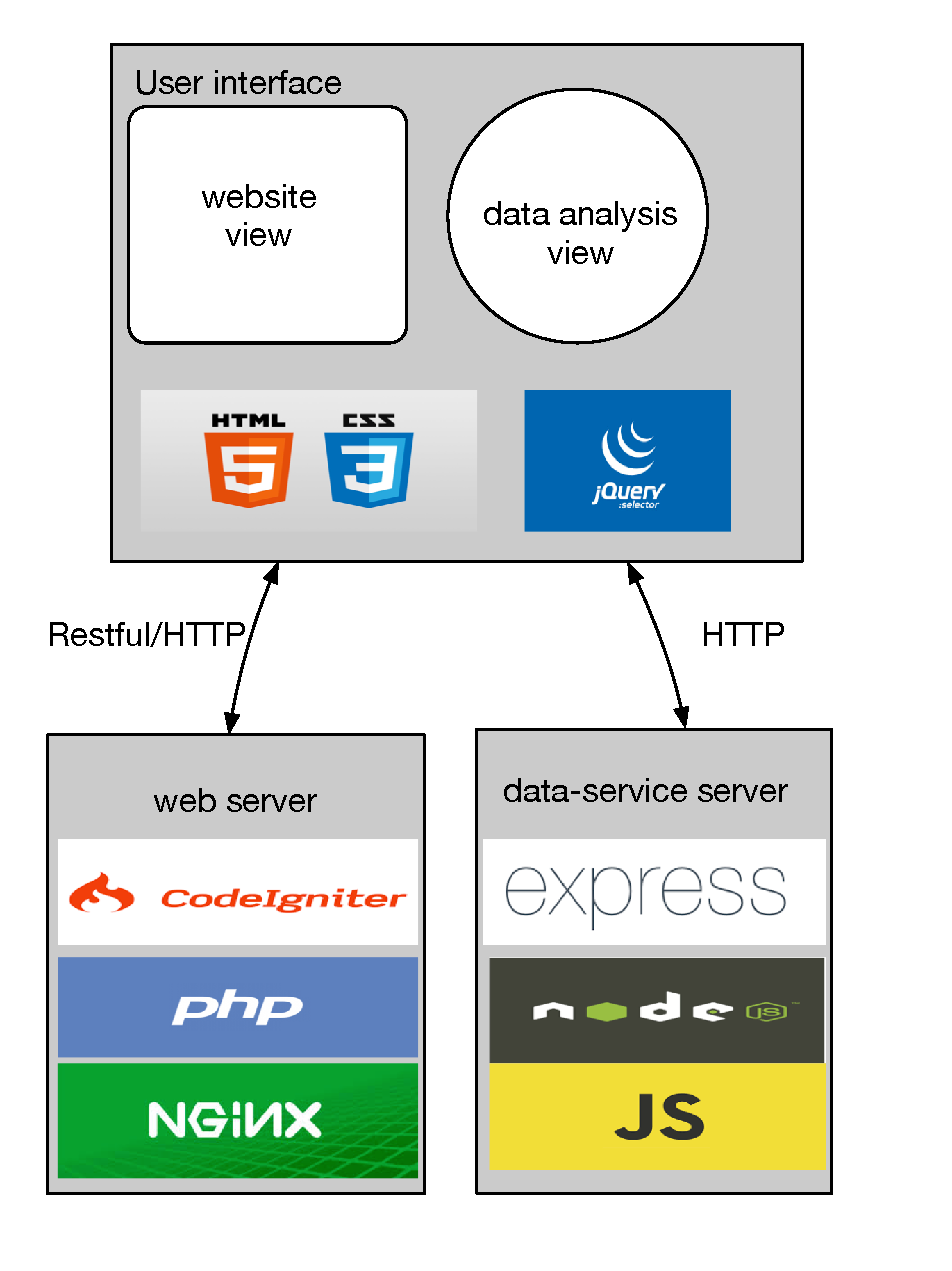
\includegraphics[width = 0.8\textwidth]{fig/layer-structure-overview.eps}
    \caption{layer structure overview}
    \label{fig:layer-overview}
\end{figure}

\section{System Architecture}
Figure \ref{fig:sys-arch} illustrates the system architecture, which shows the detail tn each parts.
The whole system is constructured from two subsystem, web server and data-service system, these two system are run independently.
Web server is a entry for user to get access to this system, throug the browser user makes requests to web server to get pages they want;
moreover it contains the most logic of web application and responsible for front-end presentation to the user.
Data-service server is a pure API-server without front-end views, which responsible for collecting user activity datas and analyze collected datas.
Whenever users interact with view element such as click buttom, click play on website embedded player, leave pages, etc. on the views provided by web servers (website view in Figure \ref{fig:layer-overview}),
a data will be sent to data-service server as a record.
After every period of time, the data in data-service server will be analyzed by our algorithm and generate refined data.
Finally, we send back the refined data back to user interface at the time users call the related api on data-service, the browser will render the result based on refined data (data analysis view in Figure \ref{fig:layer-overview}).

\begin{figure}[H]
    \centering
    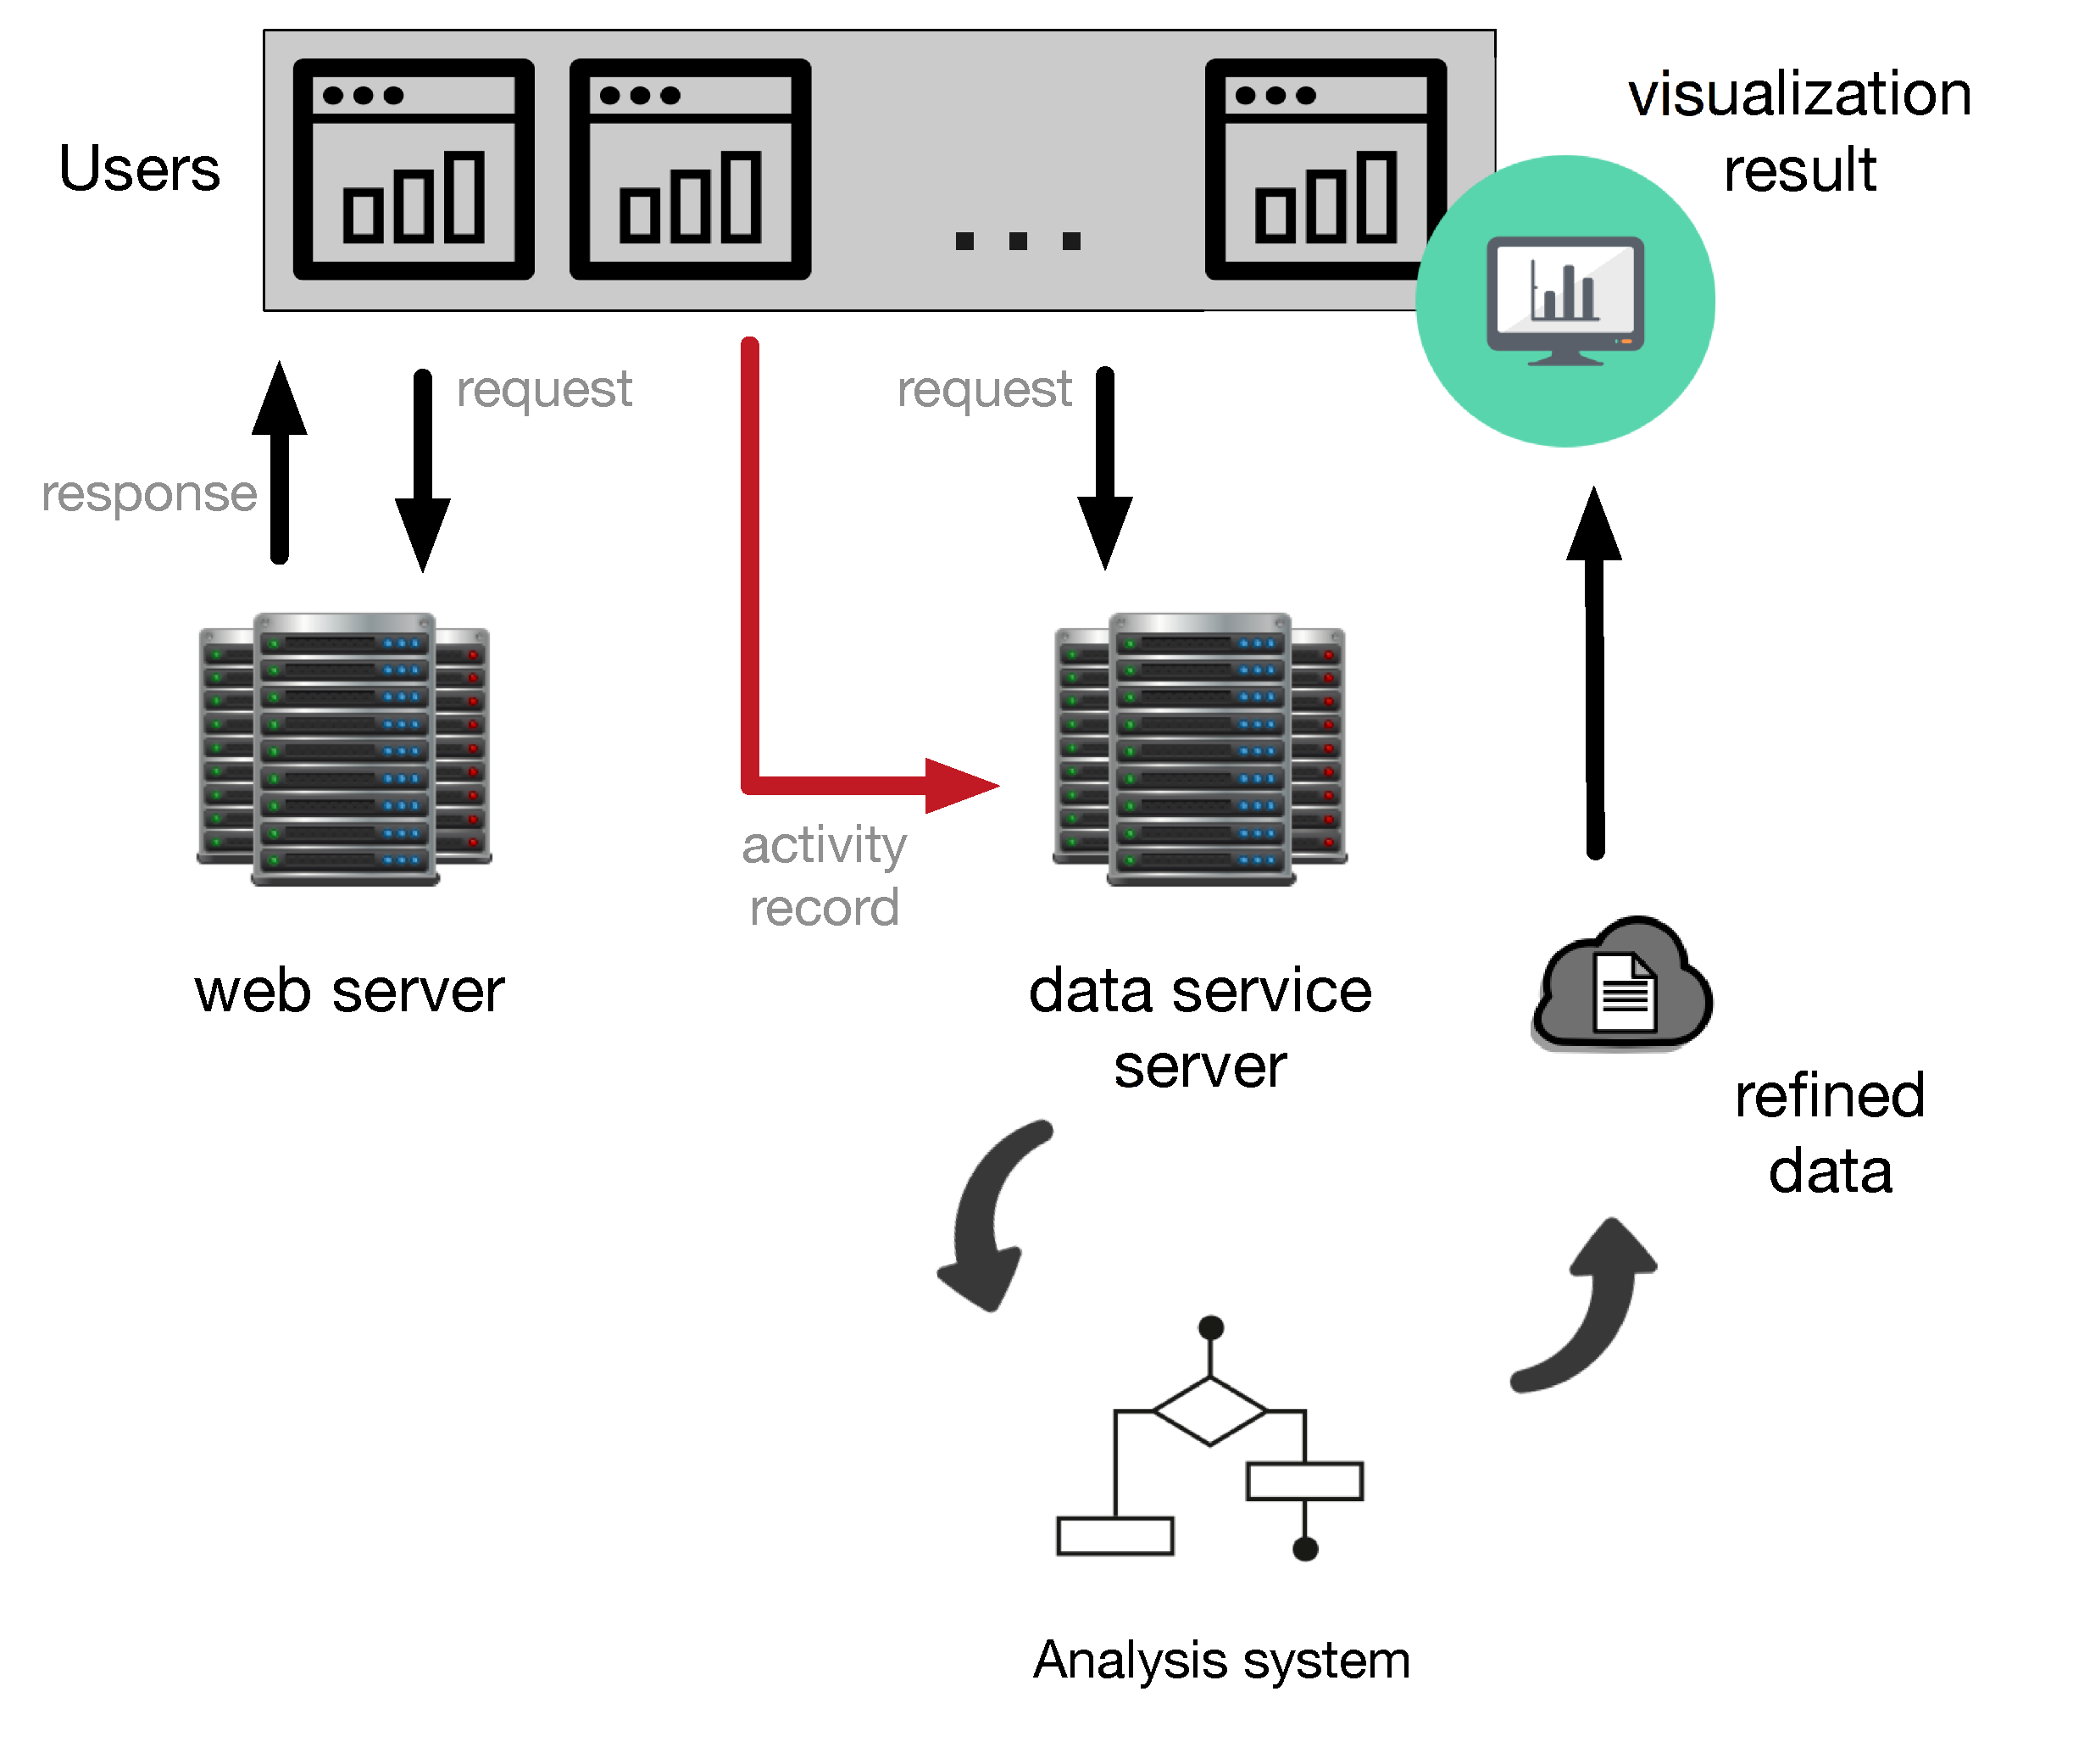
\includegraphics[width = 0.8\textwidth]{fig/system-architecture-outline.eps}
    \caption{system architecture}
    \label{fig:sys-arch}
\end{figure}

\section{User Data Flow}

\section{Website MVC Design Pattern}
MVC (Model-View-Controller) is a kind of design patter in software engineering, it seperate application into three interconnected parts, model, controller, and view \cite{Leff2001} (see Figure \ref{fig:mvc}).
Controller act as the brain of application, dealing with users' request and converts requests into command for model and view.
View provides user a Graphical User Interface (GUI) to display application's state.
Model is the only one who can access data base directly, sometimes it represents a schema of table or specification or the data type.

\begin{figure}[H]
    \centering
    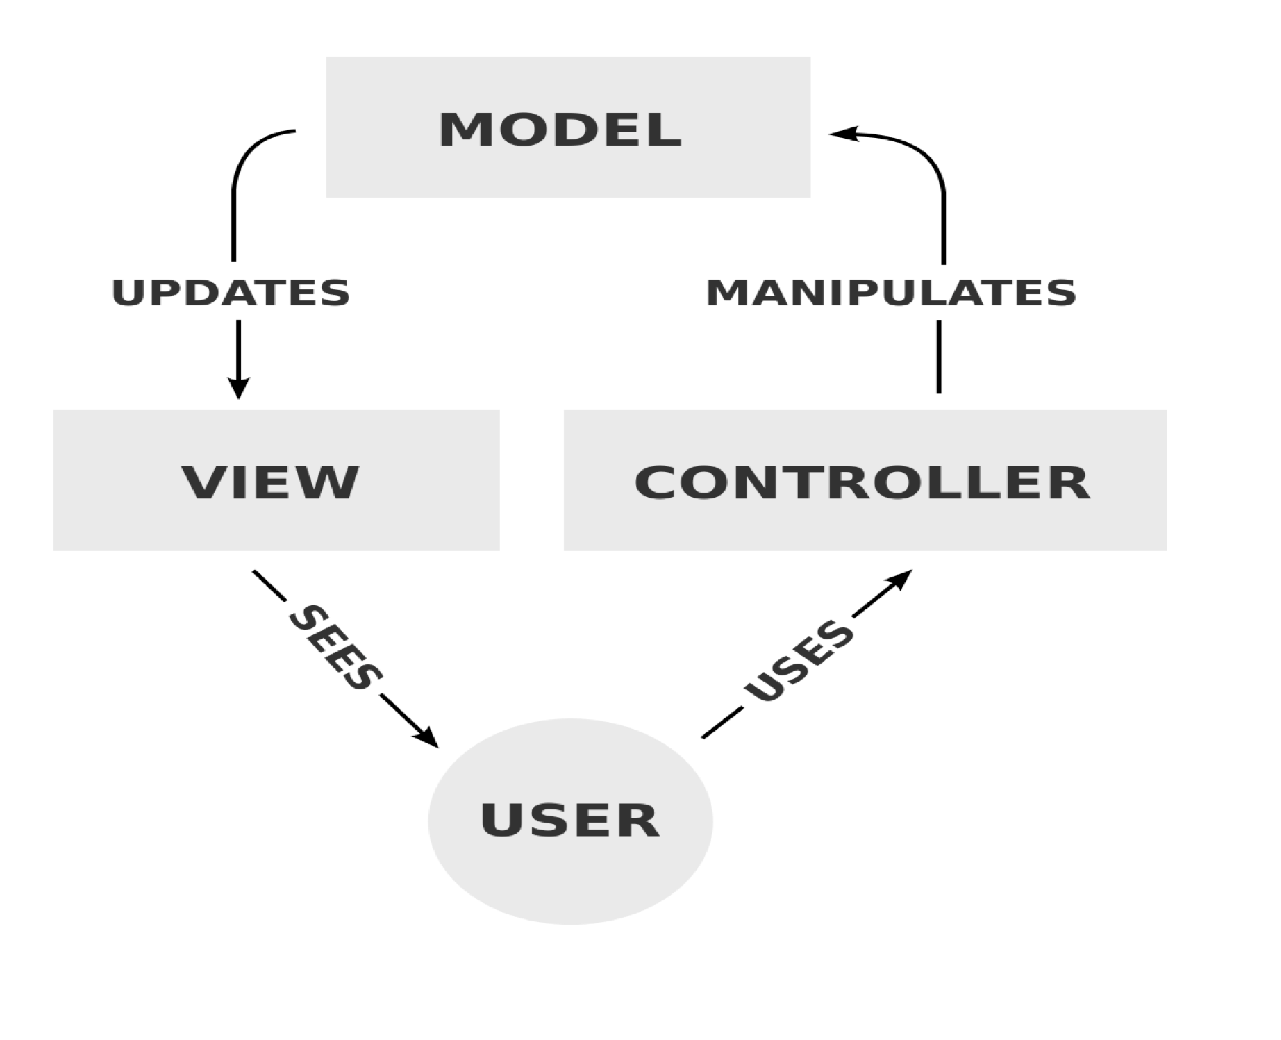
\includegraphics[width = 0.8\textwidth]{fig/mvc-relation.eps}
    \caption{Collaboration of MVC elements}
    \label{fig:mvc}
\end{figure}
